\documentclass[12pt]{report}

% import packages
\usepackage{listings}
\usepackage{xcolor}
\usepackage{graphicx}
\usepackage{amsmath}
\usepackage{hyperref}
\usepackage{geometry}
\usepackage{subfig}
\usepackage{float}
\geometry{a4paper, margin=1in}

\usepackage{pgfplots}
\pgfplotsset{compat=1.18}

\lstdefinestyle{cstyle}{
    language=C,
    basicstyle=\ttfamily\footnotesize,
    keywordstyle=\color{purple}\bfseries,
    stringstyle=\color{orange},
    commentstyle=\color{olive},
    numbers=none,
    tabsize=4,
    showspaces=false,
    showstringspaces=false,
    frame=single,
    framerule=0.8pt,
    framesep=5pt,
    aboveskip=0.5cm,
    belowskip=0.5cm,
}

\begin{document}

\title{\textbf{Bitonic Sort with MPI}}
\author{Ioannis Michalainas, Savvas Tzanetis}
\maketitle

\tableofcontents

\chapter{Abstract}
This report is part of an assignment for the \textbf{Parallel and Distributed Systems} class of the
Aristotle University's Electrical and Computer Engineering department, under professor \textit{Nikolaos Pitsianis}. 

This project implements \textit{distributed sorting} using the \textbf{Bitonic Sort} algorithm and the \textbf{Message Passing Interface (MPI)}. The primary objective is to sort a dataset of $N = 2^{(q+p)}$ numbers (where $2^p$ represents the total \textit{processes} and $2^q$ the \textit{numbers} assigned per process) utilizing inter-process communication. The implementation employs parallel processing to achieve efficient sorting, making it suitable for large-scale data sets.

\chapter{Serial Bitonic}

To grasp the concept of distributed \textbf{Bitonic Sort}, it is essential to first understand its serial implementation. This foundational knowledge will provide the necessary context for comprehending the distributed version of the algorithm.

\section{Explanation}

\textbf{Bitonic Sort} is a sorting algorithm that operates by sorting and merging bitonic sequences. A bitonic sequence is defined as a sequence of numbers that first monotonically increases and then monotonically decreases (or vise versa), or can be cyclically rotated to exhibit this pattern. Note that sorted sequences are also bitonic. For example, the sequence $6, 4, 3, 1, 2, 5, 8, 7$ is bitonic because it can be rotated to $7, 6, 4, 3, 1, 2, 5, 8$. 

The algorithm is has the following characteristics:

\begin{itemize}
    \item $log(n)$ steps, where n is the total amount of numbers, with $log(step)$ comparison phases in each step.
    \item In each comparison phase, we swap elements using the \textbf{min-max} criteria. The min-max pattern is presented in the image bellow:
\end{itemize}
\begin{figure}
    \centering
    \includegraphics[width=0.75\linewidth]{bitonic.png}
    \caption{Bitonic Sort}
    \label{fig:enter-label}
\end{figure}
\section{Example}

To illustrate the process, consider the following random sequence:
\[S\{ 3,7,4,8,6,2,1,5 \}\]
In each step each element is compared to its neighbor with distance \textbf{stage}
\begin{enumerate}
\item \textbf{Step 1, Stage 1}

\textbf{min-max pattern:} $min\:max\:max\:min\:min\:max\:max\:min$

\[
    S\{3,7,8,4,2,6,5,1\}
\]

\item \textbf{Step 2, Stage 2}

\textbf{min-max pattern:} $min\:min\:max\:max\:max\:max\:min\:min$
\[
    S\{3,4,8,7,5,6,2,1\}
\]

\item \textbf{Step 2, Stage 1}

\textbf{min-max pattern:} $min\:max\:min\:max\:max\:min\:max\:min$
\[
    S\{3,4,8,7,6,5,2,1\}
\]

\item \textbf{Step 3, Stage 3}

\textbf{min-max pattern:} $min\:min\:min\:min\:max\:max\:max\:max$
\[
    S\{3,4,2,1,6,5,7,8\}
\]

\item \textbf{Step 3, Stage 2}

\textbf{min-max pattern:} $min\:min\:max\:max\:min\:min\:max\:max$
\[
    S\{2,1,3,4,6,5,7,8\}
\]

\item \textbf{Step 3, Stage 1}

\textbf{min-max pattern:} $min\:max\:min\:max\:min\:max\:min\:max$
\[
    S\{1, 2, 3, 4, 5, 6, 7, 8\}
\]
\end{enumerate}

\section{Remarks}
\begin{enumerate}
\item The complexity of this algorithm is $O(nlog^2n)$. While it is higher than other popular sorting algorithms like \textbf{Merge Sort} or \textbf{Quick Sort},  \textbf{Bitonic Sort} is ideal for parallel implementation, because it always compares elements in a predefined sequence and the sequence of comparison does not depend on data. 
\item \textbf{Bitonic Sort} can only be used if the number of elements to sort is $2^n$. The procedure fails if the number of elements is not in the aforementioned quantity precisely.
\end{enumerate}
        
\chapter{Distributed Bitonic}
As mentioned above, this algorithm, when implemented in a serial manner, has a time complexity of \(\boldsymbol{O(n\log^2(n))}\), which is higher than most sorting algorithms. Despite that, this algorithm is useful, as it is well-suited for parallel implementations, like the one we will be discussing. For a parallel implementation, we can achieve a time complexity of \(\boldsymbol{O(\log^2(n))}\), which is significantly faster than our serial implementation. We will be achieving this goal, by utilizing the \textbf{Message Passing Interface (MPI)} for inter-process communication, allowing us to distribute the load across multiple machines.

\section{Generating Random Sequences}
The sequences we used to test our results were generated using the \textbf{rand()} function, which is part of the \textbf{C standard library}. More specifically, we selected \textit{integers} ranging from \textbf{1} to \textbf{999} for simplicity.  We use this function to create a random array of $N$ integers, which we then distribute across multiple processes.

\begin{lstlisting}[style=cstyle]
void randomVec(Vector* vec, int max) {
    srand(time(NULL));
    for (int i=0; i<vec->size; i++) {
        vec->arr[i] = rand()%max;
    }
}
\end{lstlisting}

Here, \textbf{Vector} is a \textit{struct} we implemented with two variables, \textbf{arr} for storing the data and \textbf{size} for storing the size of the array \textbf{arr}. \newpage

\section{MPI Communication}
\textbf{MPI}  allows us to simulate multiple machines, by creating multiple processes to a single computer running the same code. Each process is given an \textbf{ID} called \textbf{rank} and is generally working independently from other processes, except for times where synchronization is needed. In our code, we refer to the amount of ranks (processes) as \textbf{size}.

\begin{lstlisting}[style=cstyle]
// run a copy of main for each rank
MPI_Init(&argc, &argv);
int rank, size;
MPI_Comm_rank(MPI_COMM_WORLD, &rank);
MPI_Comm_size(MPI_COMM_WORLD, &size);
\end{lstlisting}

Processes should also be able to communicate with each other, in order to exchange data and synchronize. Luckily, the MPI library already provides us with the necessary tools:
\begin{lstlisting}[style=cstyle]
// Rank 0 Scatters data to all other ranks
MPI_Scatter(data->arr, local->size, MPI_INT, local->arr,
            local->size, MPI_INT, 0, MPI_COMM_WORLD);

// Other ranks accept data but don't send anything themselves
MPI_Scatter(NULL, local->size, MPI_INT, local->arr, 
            local->size, MPI_INT, 0, MPI_COMM_WORLD);
\end{lstlisting}

In the code above, \textbf{data} holds the randomly generated array that awaits to be sorted, while \textbf{local} represents the sub-arrays of each rank involved in the distributed sort task. 
After we perform the distributed sort, we synchronize all ranks and then gather our results to showcase them.

\begin{lstlisting}[style=cstyle]
distributed_sort(local, rank, size);
MPI_Barrier(MPI_COMM_WORLD);

[...]

MPI_Gather(local->arr, local->size, MPI_INT, sorted ? sorted->arr : NULL, 
                       local->size, MPI_INT, 0, MPI_COMM_WORLD);

// wait until all ranks reach this point
MPI_Barrier(MPI_COMM_WORLD);
results(sorted, rank, size);
\end{lstlisting}
\newpage
\section{Implementation}

In this subsection, we will discuss how the \textbf{Bitonic Sort} algorithm was implemented in a distributed manner. 

\subsection{Brief}

After each rank performs an initial sort to its local data, we enter a nested for loop. The algorithm has \textbf{p} stages, with \textbf{stage} steps each. Number of stages \textbf{p} is defined as 
$$
log_2(size)
$$
In each step, we calculate the \textbf{distance} of the \textbf{partner} we need to exchange data and said partner's rank, then we proceed to \textbf{exchange} data by following a \textbf{min} or \textbf{max} pattern. After each stage has concluded each rank sorts its local data using \textbf{elbowmerge}.

\begin{lstlisting}[style=cstyle]
initialSort(local, rank); 
for (int stage=1; stage<=p; stage++) {
    for (int step=stage; step>=1; step--) {
      int distance = 1 << (step-1);
      int partner = rank ^ distance;

      exchange(partner, local, remote);
      minmax(rank, stage, distance, local, remote);
    }
    // Ascending (0) or Descending (1)
    int direction = (rank & (1 << stage)) == 0;     
    elbowmerge(local, direction);
  }
\end{lstlisting}

Later follows a visual outline of the algorithm, illustrated featuring an example of \textbf{8} processes.

\begin{figure}
    \centering
    \includegraphics[width=1\linewidth]{distributed-algorithm.png}
    \caption{Algorithm Outline}
    \label{fig:enter-label}
\end{figure}

\subsection{Initial Sort}

First and foremost, after the random array data has been distributed evenly across all ranks, each rank will go through an \textit{initial sorting process} that will run exactly once. This sort is performed using the \textbf{qsort} function provided by the C standard library.
\begin{lstlisting}[style=cstyle]
void initialSort(Vector* local, int rank) {
  if (rank & 1) {
    qsort(local->arr, local->size, sizeof(int), compDescending);
  } else { 
    qsort(local->arr, local->size, sizeof(int), compAscending);
  }
}
\end{lstlisting}
Here \textbf{(rank \& 1)} is a logical operation equivalent to \textbf{rank} MOD \textbf{2}  that essentially allows us to sort the sub-arrays with alternating order. 
Note that the logical AND (\&) operation will be handy later on for creating alternating binary patterns, since the \textbf{Bitonic Sort} algorithm is based on \textbf{powers of 2}.

\vspace{1cm}
\begin{tabular}{|c|c|c|c|c|}
\hline
\textbf{Decimal} & \textbf{Binary} & \textbf{AND with 1} & \textbf{AND with 2} & \textbf{AND with 4} \\ \hline
0 & 000 & 000 \textit{(OFF)}& 000 \textit{(OFF)}& 000 \textit{(OFF)}\\ \hline
1 & 001 & 001 \textit{(ON)}& 000 \textit{(OFF)}& 000 \textit{(OFF)}\\ \hline
2 & 010 & 000 \textit{(OFF)}& 010 \textit{(ON)}& 000 \textit{(OFF)}\\ \hline
3 & 011 & 001 \textit{(ON)}& 010 \textit{(ON)}& 000 \textit{(OFF)}\\ \hline
4 & 100 & 000 \textit{(OFF)}& 000 \textit{(OFF)}& 100 \textit{(ON)}\\ \hline
5 & 101 & 001 \textit{(ON)}& 000 \textit{(OFF)}& 100 \textit{(ON)}\\ \hline
6 & 110 & 000 \textit{(OFF)}& 010 \textit{(ON)}& 100 \textit{(ON)}\\ \hline
7 & 111 & 001 \textit{(ON)}& 010 \textit{(ON)}& 100 \textit{(ON)}\\ \hline
\end{tabular}
\vspace{1cm}

Above, we can visualize and understand the patterns created using the logical AND ({\&}) operation for \textbf{powers of 2}.

\subsection{Data Exchange}

In this part, each process \textbf{exchanges} data with its \textbf{partner}. We need to determine the \textbf{distance} of the partner the process should exchange data with. This is given by $2^{(step-1)}$.  We then calculate the partner based on the distance \textbf{rank} XOR \textbf{step}.

The processes are arranged in a hypercube-like structure, where the rank of each process is treated as a binary number. The \textbf{XOR} operation between two binary numbers results in a number where the bits are set to 1 at positions where the two numbers differ. The distance between two nodes in a hypercube is the number of differing bits between their binary representations, known as the \textbf{Hamming distance}. 
\begin{figure}[H]
    \centering
    \includegraphics[width=0.5\linewidth]{cube.png}
    \caption{Hyper-Cube Representation}
    \label{fig:enter-label}
\end{figure}
The XOR operation helps find a partner that differs from the current process by exactly the number of bits defined by the \textit{distance} at each step. This ensures that in each stage of the algorithm, the process communicates with a partner that is located at a specific Hamming distance, consistent with the hypercube structure. At each stage, the \textit{distance} doubles (based on the step), and the \verb|rank ^ distance| operation calculates a process ID that is at the desired Hamming distance.

\vspace{1cm}
\begin{tabular}{|c|c|c|c|c|}
\hline
\textbf{Decimal} & \textbf{Binary} & \textbf{XOR with 1} & \textbf{XOR with 2} & \textbf{XOR with 4} \\ \hline
0 & 000 & 001 & 010 & 100 \\ \hline
1 & 001 & 000 & 011 & 101 \\ \hline
2 & 010 & 011 & 000 & 110 \\ \hline
3 & 011 & 010 & 001 & 111 \\ \hline
4 & 100 & 101 & 110 & 000 \\ \hline
5 & 101 & 100 & 111 & 001 \\ \hline
6 & 110 & 111 & 100 & 010 \\ \hline
7 & 111 & 110 & 101 & 011 \\ \hline
\end{tabular}
\vspace{1cm}
        
Every rank then sends their \textbf{local} array to their respective partner and receive their partners data in a buffer called \textbf{remote}.

\begin{lstlisting}[style=cstyle]
void exchange(int partner, Vector* local, Vector* remote) {

  MPI_Sendrecv(local->arr, local->size, MPI_INT, partner, 0,
               remote->arr, local->size, MPI_INT, partner, 0,
               MPI_COMM_WORLD, MPI_STATUS_IGNORE);
}
\end{lstlisting}

\subsection{Min-Max Operations}

This part of the algorithm involves processing the data each rank receives from its partner.  Each rank compares all the local elements to the remote ones element-wise and keeps the \textbf{min} or \textbf{max} elements, depending on the stage and the distance at the specific point of the algorithm. 

A helpful way to visualize the criteria for choosing min or max is to imagine that for each stage \textit{mirrors} are placed before the processes with ranks $2^{stage} + k*w$ where $w=2*mirror$ and k any natural number $N[0,1,2,...]$, spanning the whole array of processes. We then determine in which mirrors province does the rank we examine belong and calculate its distance from the mirror, its \textit{reflection}.

Let's examine the example of 8 processes to clarify our approach. Suppose we are on the \textbf{first stage} with \textbf{distance one}. We place \textit{mirrors} at positions \textbf{2} and \textbf{6}, like so: $[p0\:p1|p2\:p3,p4\:p5|p6\:p7]$. In this case, $p0,p3,p4,p7$ would have a \textit{reflection} (distance from the mirror) of 1 and $p1,p2,p5,p6$ a \textit{reflection} of 0. The required min max order is: $[min\:max | max\:min, min\:max | max\:min]$.  We notice that there is symmetry around the locations of the mirrors, spanning $w=2*mirror$ range. Employing a similar binary pattern creation tactic we used for the initial sort, we determine whether a process should keep the min or the max elements element wise. We concluded to the following formula:
$$
reflection\:\&\: 2^{(log_2(distance))}
$$
If the above operation results to 0, we get a \textbf{max} element-wise comparison, else we get a \textbf{min} element-wise comparison.

This approach generalizes for any number of processes that is a \textbf{power of 2}.
\newpage
\begin{lstlisting}[style=cstyle]
void minmax(int rank, int stage, int distance, 
            Vector* local, Vector* remote) {
  int mirror = 1 << stage;
  int w = 2*mirror;
  int pos = rank % w;

  int reflection = pos<mirror ? mirror-pos - 1 : pos-mirror; 

  if (reflection & (1 << (int)log2(distance))) {
    min(local, remote);
  } else {
    max(local, remote);
  }
}
\end{lstlisting}

        \subsection{Elbow Merge}
        
        Lastly,  \textbf{elbowmerge} is a sorting technique specific to bitonic sequences (that being the reason why we do not use it for our initial sort, as the arrays are arbitrary). 
        
        We first begin by identifying the \textbf{extremum} of the bitonic array, either the \textbf{maximum} (elbow) or the \textbf{minimum} (pit). To do that, we need to locate a point in the sequence that its adjacent points (in the context of a circular buffer) are either both smaller than said point (elbow) or larger (pit). 
        
        If we do not manage to find such point, it means that the sequence is of the form $[a, a, b, b]$ or $[b, b, a, a]$ or $[a, a, a, a]$ where $a>b$. Such sequences are not considered bitonic, but consist a possible input for the elbow function. To handle them gracefully, we select the max element by convention and return it as the elbow. 
        
        That way, locating the extremum of a bitonic sequence is performed in $O(n)$ time, even for the corner cases.
        \newpage

        \begin{lstlisting}[style=cstyle] 
        
        Extremum elbow(Vector* local) {

  Extremum point;
  point.index = -1;
  point.polarity = 0;

  int  n   = local->size;
  int* arr = local->arr;

  for (int i=0; i<n; i++) {
    int prev = arr[(i-1 + n) % n];
    int curr = arr[i];
    int next = arr[(i+1) % n];

    if (curr>prev && curr>next) {
      point.index = i;
      point.polarity = 1;
      return point; // elbow
    }

    if (curr<prev && curr<next) {
      point.index = i;
      point.polarity = -1;
      return point; // pit
    }
  }

  // invalid bitonic sequences (corner cases)
  int max = 0;
  for (int i=1; i<n; i++) {
    if (arr[i] > arr[max]) {
      max = i;
    }
  }
  // return max as elbow
  point.index = max;
  point.polarity = 1;

  return point;
}
            
\end{lstlisting}
After identifying the \textbf{extremum}, we add it either on the end or the start of a temporary array, depending on if we have a \textbf{minimum} or a \textbf{maximum}. For the \textbf{elbow} case, we then compare the values of the \textbf{left} and \textbf{right} indices and the one containing the largest element gets to be placed next in the temporary array and shift its index by one (-1 for left +1 for right) in a circular buffer manner. This processes is repeated until all elements are placed in the tmp array, resulting in a fully sorted array, and follows commensurable logic in the \textbf{pit} case. If we want to sort the array in \textbf{ascending} order we \textit{directly} copy tmp to local, if we want \textbf{descending} order we \textit{reverse} copy our results. 
\newpage
\begin{lstlisting}[style=cstyle]
void elbowmerge(Vector* local, int direction) {
  Extremum point = elbow(local);
  int  n   = local->size;
  int* tmp = malloc(sizeof(int)*n);

  int left  = (point.index-1 + n) % n;
  int right = (point.index+1) % n;

  if (point.polarity == -1) {  
    int i = 0;
    tmp[i++] = local->arr[point.index];  

    while (i < n) {
      if (local->arr[left] < local->arr[right]) {
        tmp[i++] = local->arr[left];
        left = (left-1 + n) % n;  // move left index circularly
      } else {
        tmp[i++] = local->arr[right];
        right = (right + 1) % n;  // move right index circularly
      }
    }
  } else if (point.polarity == 1) {  
    int i = n-1;
    tmp[i--] = local->arr[point.index];  

    while (i >= 0) {
      if (local->arr[left] > local->arr[right]) {
        tmp[i--] = local->arr[left];
        left = (left-1 + n) % n;  // move left index circularly
      } else {
        tmp[i--] = local->arr[right];
        right = (right+1) % n;  // move right index circularly
      }
    }
  }
  if (direction == 1) {
    memcpy(local->arr, tmp, sizeof(int)*n);
  } else {
    for (int j=0; j<n; j++) {
      local->arr[j] = tmp[n-1 - j];
    }
  }
  free(tmp);
}


\end{lstlisting}
The merging process is also performed in $O(n)$ time, making the total computational cost of the local sort $O(n)$ too.

\chapter{Results}
As previously mentioned, a serial version of this algorithm has a times complexity of \(\boldsymbol{O(n \log^2(n))}\), which is not ideal, as there are faster algorithms, but a parallel or distributed version, significantly lessens this to \(\boldsymbol{O(\log^2(n))}\).

We tested these algorithms with \textbf{33.554.432} (or $2^{25}$) random numbers in a sequence, ranging between the numbers \textbf{1 - 999}.  Note that the bitonic sorting algorithm can successfully sort only sequences in the \textbf{power of 2}. We verified correctness by using \textbf{qsort}.

The algorithms where run inside the \textbf{Aristotle Cluster} provided by the \textbf{Aristotle University of Thessaloniki}, with \textbf{4 cores}, splitting the load among \textbf{4 processes} or \textbf{ranks.}

\begin{table}[h!]
    \centering
    \begin{tabular}{|c|c|c|c|}
        \hline
        \rule{0pt}{3ex}\textbf{Performance Table} & \textbf{Serial}                 & \textbf{Distributed}          & \textbf{Quick Sort}          \\ \hline
        \rule{0pt}{3ex}Time Complexity            & \(\boldsymbol{O(n \log^2(n))}\) & \(\boldsymbol{O(\log^2(n))}\) & \(\boldsymbol{O(n\log(n))}\) \\ \hline
        \rule{0pt}{3ex}Time& \textbf{1}min \textbf{51}sec    & \textbf{6.02}sec              & \textbf{1}min \textbf{24}sec \\ \hline
    \end{tabular}
    \caption{Performance Table.}
    \label{tab:simple_table}
\end{table}

\begin{center}
    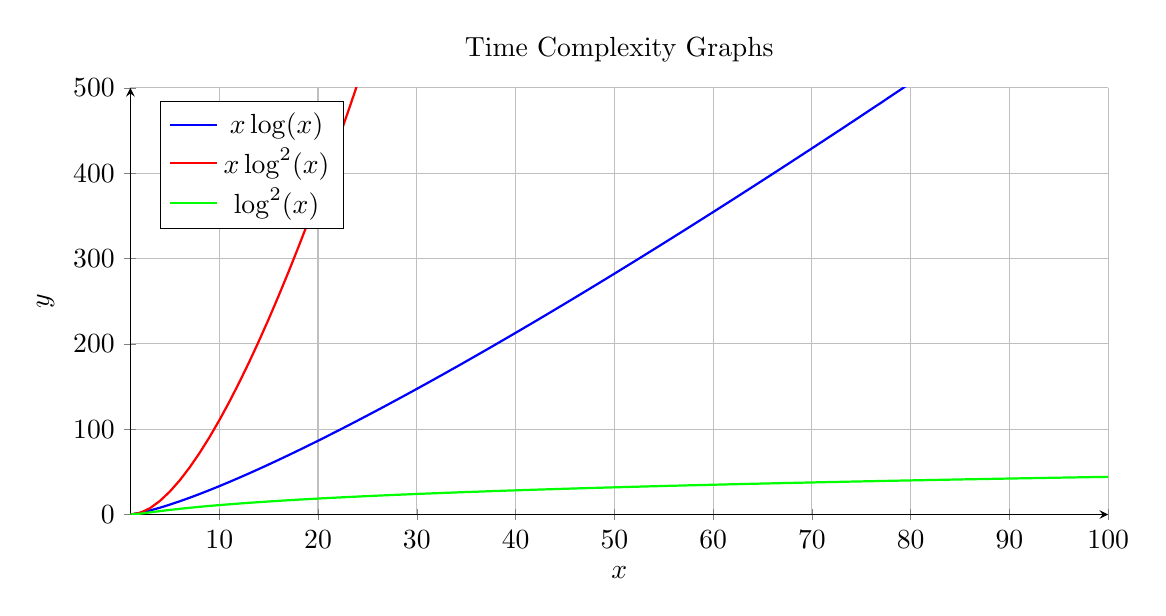
\begin{tikzpicture}
        \begin{axis}[
            width=14cm,
            height=7cm,
            xlabel={$x$},
            ylabel={$y$},
            xmin=1, xmax=100,
            ymin=0, ymax=500,
            legend pos=north west,
            grid=major,
            axis x line=bottom,
            axis y line=left,
            title={Time Complexity Graphs}
        ]
            % plot x * log2(x)
            \addplot[blue, thick] expression[domain=1:100, samples=100]{x * ln(x)/ln(2)};
            \addlegendentry{$x \log(x)$}

            % plot x * (log2(x))^2
            \addplot[red, thick] expression[domain=1:100, samples=100]{x * (ln(x)/ln(2))^2};
            \addlegendentry{$x \log^2(x)$}

            % plot (log2(x))^2
            \addplot[green, thick] expression[domain=1:100, samples=100]{(ln(x)/ln(2))^2};
            \addlegendentry{$\log^2(x)$}
        \end{axis}
    \end{tikzpicture}
\end{center}
As we can see our distributed implementation of the \textbf{Bitonic Sort} algorithm is significantly faster than a serial implementation, as well as other serial sorting algorithms like \textbf{Quick Sort}.

\chapter{Tools and Sources}
In this project, the following tools where used:
\begin{enumerate}
\item The \textbf{C} programming language.
\item The \textbf{OpenMPI} Library for implementing the distributed algorithm.
\item The \textbf{Neovim} text editor for development.
\item \textbf{Gimp} for asset creation.
\item \textbf{GitHub} for version control.
\item \textbf{GitHub Copilot} as an AI assistant.
\end{enumerate}
While the following sources were helpful in understanding of the problem presented in the assignment.
\begin{itemize}
\item \url{https://en.wikipedia.org/wiki/Bitonic_sorter}
\item \url{https://www.geeksforgeeks.org/bitonic-sort/}
\item \url{https://www.open-mpi.org/doc/v4.0/}
\item Lecture notes from the \textbf{Parallel and Distributed Systems} course, written by professor \textbf{Nikolaos Pitsianis}.
\item Credits to \textit{Epameinondas Bakoulas} for keeping lecture notes and creating the distributed-algorithm.png asset.
\end{itemize}

\end{document}